\documentclass[a4paper, 11pt]{article}

% --- Packages ---
\usepackage[left=1.7cm, right=1.7cm, top=1.8cm, bottom=1.7cm]{geometry}
\usepackage{graphicx}
\usepackage[table]{xcolor}
\usepackage{hyperref}
\usepackage{booktabs}
\usepackage{tabularx}
\usepackage{longtable}
\usepackage{fancyhdr}
\usepackage{titlesec}
\usepackage{array}
\usepackage{caption}

% --- Hyperlink Setup ---
\hypersetup{
    colorlinks=true,
    linkcolor=black,
    urlcolor=blue,
    pdftitle={QuickBites Transaction Reliability Report}
}

% --- Header and Footer Setup ---
\pagestyle{fancy}
\fancyhf{}
\renewcommand{\headrulewidth}{0pt}
\renewcommand{\footrulewidth}{0.4pt}
\fancyfoot[L]{\footnotesize QuickBites - Transaction Reliability Assignment}
\fancyfoot[R]{\thepage}

% --- Custom Table Row Colors ---
\definecolor{HeaderGray}{HTML}{E6E6E6}

\setlength{\parskip}{0.45em}
\setlength{\parindent}{0pt}

\begin{document}

% ==========================================
% COVER PAGE
% ==========================================
\begin{titlepage}
    \centering
    \vspace*{4.2cm}

    {\Huge \bfseries QuickBites \par}
    \vspace{0.2cm}
    {\Large \bfseries Transaction Reliability and Robustness Report \par}
    \vspace{0.7cm}

    {\large Module B Assignment \par}
    {\large Date: \today \par}
    \vspace{1.1cm}

    \begin{center}
    \renewcommand{\arraystretch}{1.5}
    \begin{tabular}{|p{7.2cm}|p{8.0cm}|}
    \hline
    \rowcolor{HeaderGray}
    \textbf{Team Members} & \textbf{Role} \\ \hline
    Bhavya Parmar & Backend and Database Design \\ \hline
    Surriya Gokul & SQL Indexing and Benchmarking \\ \hline
    Sonagiri Thoshith Kautilya & Frontend and UI or UX \\ \hline
    \end{tabular}
    \end{center}
    \vspace{0.9cm}

    {\large GitHub: \href{https://github.com/mohit-codes-21/QuickBites}{https://github.com/mohit-codes-21/QuickBites} \par}
    {\large Video: \href{https://drive.google.com/file/d/11_qTASPAAZiH_r3rJKdd1T1OuKAl3c3_/view?usp=sharing}{View Submission Video} \par}
    \vspace{1.5cm}

    {\large Indian Institute of Technology Gandhinagar \par}
    \vfill
\end{titlepage}

% ==========================================
% TABLE OF CONTENTS
% ==========================================
\newpage
\tableofcontents
\newpage

% ==========================================
% REPORT CONTENT
% ==========================================

\section{Introduction}
This report documents reliability verification for QuickBites under concurrent usage, race pressure, injected failures, and sustained load. The objective is to validate transaction behavior against ACID principles and assignment criteria: correctness of outcomes, rollback safety, multi-user isolation, and robustness under stress.

\section{Verification Scope and Evaluation Criteria}
The verification scope covers five suites: concurrent usage, race condition testing, failure simulation, ACID checks, and stress testing. Evaluation focused on four properties:
\begin{itemize}
    \item \textbf{Atomicity:} operations either commit fully or rollback fully.
    \item \textbf{Consistency:} no invalid relational states, including orphan references or incomplete entities.
    \item \textbf{Isolation:} one user flow cannot corrupt or leak partial state into another.
    \item \textbf{Durability:} committed data persists across process restarts.
\end{itemize}

\section{Implementation Controls for Correctness}

\subsection{Transaction and rollback discipline}
Critical write paths execute in explicit transaction boundaries with commit-on-success and rollback-on-exception behavior. Failure tests intentionally inject partial-signup and partial-request conditions to verify that incomplete entities are not persisted.

\subsection{Concurrency and race hardening}
Race-sensitive operations are serialized using lock-backed techniques on shared resources such as customer carts and order assignment. Observed outcomes confirm one-winner behavior in race scenarios, with deterministic final state under contention.

\subsection{Data integrity and observability}
Database constraints and audit logs provide secondary integrity protection and post-run traceability. All suites emit structured metrics to CSV and JSONL for repeatable analysis and reporting.

\section{Experimental Setup and Test Scenarios}
Experiments were executed with Python test scripts and Locust against the local API service. The table below maps each suite to scenario intent and verification target.

\vspace{0.3cm}
\renewcommand{\arraystretch}{1.3}
\begin{tabularx}{\textwidth}{|l|l|X|X|}
\hline
\rowcolor{HeaderGray}
\textbf{Suite} & \textbf{Primary Script} & \textbf{Scenario Focus} & \textbf{Verification Target} \\ \hline
Concurrent & \texttt{tests/concurrent\_test.py} & Parallel reads and same-record writes & Isolation and non-interference \\ \hline
Race & \texttt{tests/race\_condition\_test.py} & Simultaneous signup and delivery acceptance & Single correct winner \\ \hline
Failure & \texttt{tests/failure\_simulation\_test.py} & Timeouts and forced disconnects & Rollback and no partial state \\ \hline
ACID & \texttt{tests/acid\_verification.py} & Atomicity, consistency, isolation, durability & Property-level pass or fail \\ \hline
Stress & \texttt{tests/stress\_test.py} and \texttt{locustfile.py} & High request volume and mixed CRUD & Correctness plus latency behavior \\ \hline
\end{tabularx}

\section{Required Reliability Explanations}

\subsection{How correctness of operations is ensured}
Correctness is enforced through explicit transaction boundaries for critical writes, with commit on success and rollback on any failure path. Data integrity is further protected using relational constraints and post-operation validation checks. ACID verification scenarios confirm atomicity, consistency, isolation, and durability at the behavior level, not only at code level. Structured logs and metrics provide traceability so each claim can be tied to reproducible evidence.

\subsection{How failures are handled}
Failure handling follows a fail-safe pattern: if a write cannot complete safely, the transaction is aborted and rolled back. Timeout and forced-disconnect simulations verify that partial entities are not left behind. Mid-transaction fault injection during signup confirms that invalid partial users cannot authenticate afterward. This approach ensures the system prefers rollback over inconsistent partial commit.

\subsection{How multi-user conflicts are handled}
Multi-user conflicts are managed using serialization controls on race-sensitive resources (for example, shared cart updates and delivery acceptance). In signup races, only one request is allowed to succeed for the contested identity while competing requests are rejected or rolled back. In delivery acceptance races, one-winner behavior is preserved and duplicate assignment is prevented. These checks were validated under concurrent thread pressure and repeated contention.

\subsection{What experiments were performed}
The following experiments were executed for this report:
\begin{itemize}
    \item Concurrent usage: four scenarios including 15 parallel reads, 15 parallel updates, delete-while-readers, and 25-way cart contention.
    \item Race conditions: 50 concurrent signup contenders and 10 concurrent delivery acceptance contenders.
    \item Failure simulation: three injected fault modes (mid-transaction rollback, timeout handling, forced disconnect).
    \item ACID verification: atomicity, consistency, isolation, and durability checks including restart durability.
    \item Stress testing: threading workload of 1000 requests across 40 threads and Locust headless run with 60 users (latest aggregate 3652 requests).
\end{itemize}

\subsection{Observations and limitations}
Observed behavior is robust: all latest test entries passed, and both stress modes reported zero request failures in the latest run set. The main performance limitation is elevated tail latency on write-heavy paths compared with read-heavy paths under contention. Additional limitations include local-environment benchmarking (single-machine, development server context), synthetic workload distributions, and the absence of multi-node deployment effects. Therefore, the results are strong for assignment-grade reliability validation but should be complemented with production-style load profiling for final capacity planning.

\section{Results and Analysis}

\subsection{Scenario scale and created-entity counts}
To make concurrency and race outcomes explicit, Table~\ref{tab:scenario-scale} summarizes how many users, workers, contenders, or requests were involved in each scenario, and what entities were actually created versus rolled back.

\renewcommand{\arraystretch}{1.25}
\begin{table}[h]
\centering
\begin{tabularx}{\textwidth}{|p{4.1cm}|p{4.0cm}|p{4.4cm}|X|}
\hline
\rowcolor{HeaderGray}
\textbf{Scenario} & \textbf{Load Scale} & \textbf{Created / Rolled Back} & \textbf{Observed Outcome} \\ \hline
Concurrent S1 (parallel reads) & 15 reader threads & No new entities (read-only) & successful\_reads = 15/15 \\ \hline
Concurrent S2 (parallel updates) & 15 updater threads & No new entities; one final item version & updates\_ok = 15/15 \\ \hline
Concurrent S3 (delete while reading) & 14 readers + 1 deleter & No new entities; target record removed from active listing & readers = 14, post\_visible = 0 \\ \hline
Concurrent S4 (cart contention) & 25 concurrent updates & No new users/items; cart quantity converged correctly & updates\_ok = 25/25 \\ \hline
Race signup & 50 simultaneous signup attempts & Users created = 1, rolled back = 49 & single active user row after race \\ \hline
Race delivery acceptance & 10 delivery contenders & Winning assignments = 1 & one-winner invariant maintained \\ \hline
Failure simulation suite & 3 injected failure scenarios & Partial users/accounts created = 0 & rollback preserved consistency in all 3 cases \\ \hline
Stress (threading script) & 1000 requests across 40 threads & Temporary menu records created and cleaned = 187 & error\_rate = 0.000\% \\ \hline
Stress (Locust headless) & 60 simulated users, 3652 requests & Login sessions observed = 60, failures = 0 & sustained mixed CRUD with 0 failures \\ \hline
\end{tabularx}
\caption{Scenario participation scale and created-entity outcomes from latest run artifacts.}
\label{tab:scenario-scale}
\end{table}

\vspace{0.2cm}
\noindent These counts show that race-heavy user creation paths were stress-tested with high contention, while rollback behavior prevented duplicate or partial writes.

\subsection{Suite-level outcomes}
\renewcommand{\arraystretch}{1.3}
\begin{tabular}{|p{3.2cm}|p{2.0cm}|p{2.0cm}|p{2.0cm}|p{3.8cm}|}
\hline
\rowcolor{HeaderGray}
\textbf{Suite} & \textbf{Total} & \textbf{Passed} & \textbf{Failed} & \textbf{Pass Rate} \\ \hline
acid & 5 & 5 & 0 & 100.00\% \\ \hline
concurrent & 4 & 4 & 0 & 100.00\% \\ \hline
failure & 4 & 4 & 0 & 100.00\% \\ \hline
race & 2 & 2 & 0 & 100.00\% \\ \hline
stress & 1 & 1 & 0 & 100.00\% \\ \hline
\end{tabular}

\vspace{0.2cm}
\footnotesize Overall latest status: \textbf{16/16} test entries passed (\textbf{100.00\%}).
\normalsize

\subsection{Detailed latest test entries}
\small
\renewcommand{\arraystretch}{1.2}
\begin{longtable}{|p{3.8cm}|p{1.4cm}|p{1.3cm}|p{1.7cm}|p{2.8cm}|p{4.6cm}|}
\hline
\rowcolor{HeaderGray}
\textbf{Test Case} & \textbf{Suite} & \textbf{Status} & \textbf{Duration (ms)} & \textbf{Parallel users/ops} & \textbf{Result Detail} \\ \hline
\endfirsthead

\hline
\rowcolor{HeaderGray}
\textbf{Test Case} & \textbf{Suite} & \textbf{Status} & \textbf{Duration (ms)} & \textbf{Parallel users/ops} & \textbf{Result Detail} \\ \hline
\endhead

ACID Atomicity & acid & PASS & 749.684 & 1 client write flow & Signup rejected as expected after injected fault; no partial user visible. \\ \hline
ACID Consistency & acid & PASS & 532.453 & 1 client, 4 write ops & Integrity checks show zero orphan orders, order-items, and customers. \\ \hline
ACID Durability & acid & PASS & 1425.692 & 1 commit + restart verify & Committed record remained visible after controlled service restart. \\ \hline
ACID Isolation & acid & PASS & 423.972 & 2 parallel actors & No dirty visibility observed during partial write and disconnect window. \\ \hline
ACID Summary & acid & PASS & 3421.197 & Aggregate of 4 checks & Aggregate ACID status: 4/4 checks passed. \\ \hline
Concurrent Scenario 1 - 15 parallel reads & concurrent & PASS & 866.930 & 15 parallel readers & All 15 reads completed successfully under parallel execution. \\ \hline
Concurrent Scenario 2 - 15 parallel updates & concurrent & PASS & 924.887 & 15 parallel updaters & All updates succeeded; final state converged to a valid latest write. \\ \hline
Concurrent Scenario 3 - delete while readers run & concurrent & PASS & 887.844 & 14 readers + 1 deleter & Readers stayed stable while delete completed; post-delete visibility is zero. \\ \hline
Concurrent Scenario 4 - same cart item contention & concurrent & PASS & 1045.663 & 25 parallel cart updates & Quantity updates serialized correctly; no corruption under 25 parallel writes. \\ \hline
Failure Simulation Summary & failure & PASS & 2673.148 & Aggregate of 3 tests & Failure suite aggregate status: 3/3 scenarios passed. \\ \hline
Failure Test 1 - Mid-transaction rollback & failure & PASS & 790.622 & 1 signup operation & Signup aborted and rollback verified; account remains non-authenticatable. \\ \hline
Failure Test 2 - API timeout simulation & failure & PASS & 937.499 & 1 timeout operation & Timeout handling preserved prior consistent state; no partial record written. \\ \hline
Failure Test 3 - Forced disconnect mid-write & failure & PASS & 907.160 & 1 partial-write sender & Connection interruption did not leave partially committed user/account rows. \\ \hline
Race Condition - 50 concurrent signup attempts & race & PASS & 12979.271 & 50 concurrent contenders & Exactly one successful signup; remaining contenders rolled back cleanly. \\ \hline
Race Condition - concurrent delivery acceptance & race & PASS & 1515.869 & 10 delivery contenders & Single delivery partner accepted order; one-winner invariant maintained. \\ \hline
Stress Test (threading fallback) & stress & PASS & 21939.766 & 40 threads, 1000 ops & 1000 requests, 0.000\% errors, avg 870.285 ms, median 670.651 ms, p95 2471.012 ms. \\ \hline
\end{longtable}
\normalsize

\subsection{Stress and load comparison}
\renewcommand{\arraystretch}{1.3}
\begin{tabularx}{\textwidth}{|X|p{5.7cm}|p{5.7cm}|}
\hline
\rowcolor{HeaderGray}
\textbf{Metric} & \textbf{Threading Stress Script} & \textbf{Locust Headless Run} \\ \hline
Total requests & 1000 & 3652 \\ \hline
Error or failure rate & 0.000\% & 0.000\% \\ \hline
Average response time & 870.285 ms & 380.101 ms \\ \hline
P95 response time & 2471.012 ms & 840.000 ms \\ \hline
Median response time & 670.651 ms & 310.000 ms \\ \hline
Throughput & 45.579 req/s & 58.775 req/s \\ \hline
\end{tabularx}

\subsection{Endpoint-level latency summary}
\small
\renewcommand{\arraystretch}{1.2}
\begin{longtable}{|p{5.8cm}|p{1.6cm}|p{1.9cm}|p{1.9cm}|p{1.7cm}|p{1.5cm}|}
\hline
\rowcolor{HeaderGray}
\textbf{Endpoint} & \textbf{Source} & \textbf{Avg (ms)} & \textbf{P95 (ms)} & \textbf{Error (\%)} & \textbf{RPS} \\ \hline
\endfirsthead

\hline
\rowcolor{HeaderGray}
\textbf{Endpoint} & \textbf{Source} & \textbf{Avg (ms)} & \textbf{P95 (ms)} & \textbf{Error (\%)} & \textbf{RPS} \\ \hline
\endhead

\texttt{GET /api/menu-items} & Threading & 881.842 & 1422.253 & 0.000 & 14.038 \\ \hline
\texttt{GET /api/menu-items?search=single} & Threading & 317.413 & 453.526 & 0.000 & 12.762 \\ \hline
\texttt{POST /api/menu-items} & Threading & 1624.641 & 3653.763 & 0.000 & 8.523 \\ \hline
\texttt{PUT /api/menu-items/<rid>/<iid>} & Threading & 991.745 & 2976.474 & 0.000 & 4.968 \\ \hline
\texttt{DELETE /api/menu-items/<rid>/<iid>} & Threading & 843.913 & 2596.822 & 0.000 & 5.287 \\ \hline
\texttt{DELETE /api/menu-items/<rid>/<iid>} & Locust & 297.508 & 510.000 & 0.000 & 10.976 \\ \hline
\texttt{GET /api/menu-items} & Locust & 525.616 & 870.000 & 0.000 & 14.806 \\ \hline
\texttt{GET /api/menu-items?search=single} & Locust & 222.189 & 370.000 & 0.000 & 16.046 \\ \hline
\texttt{POST /api/menu-items} & Locust & 518.796 & 1400.000 & 0.000 & 10.622 \\ \hline
\texttt{PUT /api/menu-items/<rid>/<iid>} & Locust & 274.287 & 450.000 & 0.000 & 5.359 \\ \hline
\end{longtable}
\normalsize

\section{Visual Evidence}

\begin{figure}[h]
    \centering
    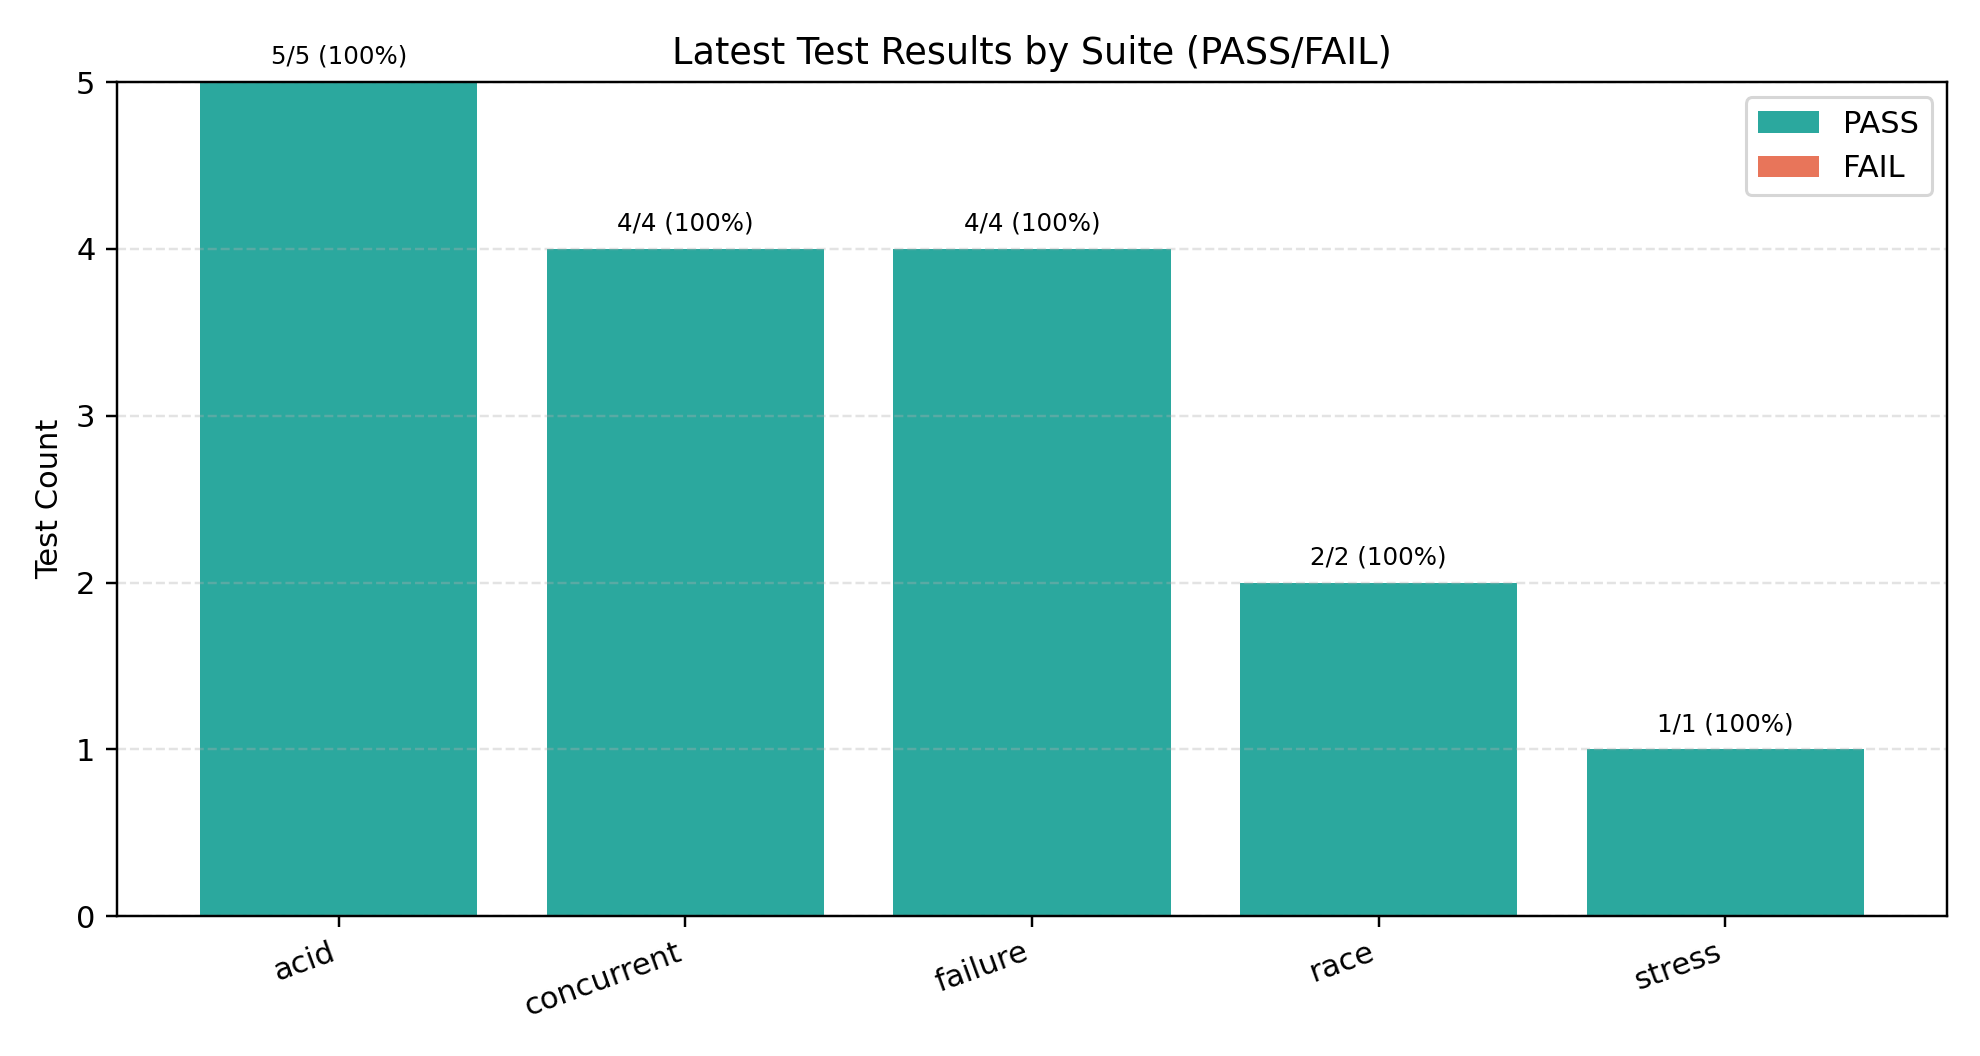
\includegraphics[width=0.84\textwidth]{../figures/test_cases/test_pass_fail_by_suite.png}
    \caption{Figure 1: PASS and FAIL distribution by suite.}
\end{figure}

\begin{figure}[h]
    \centering
    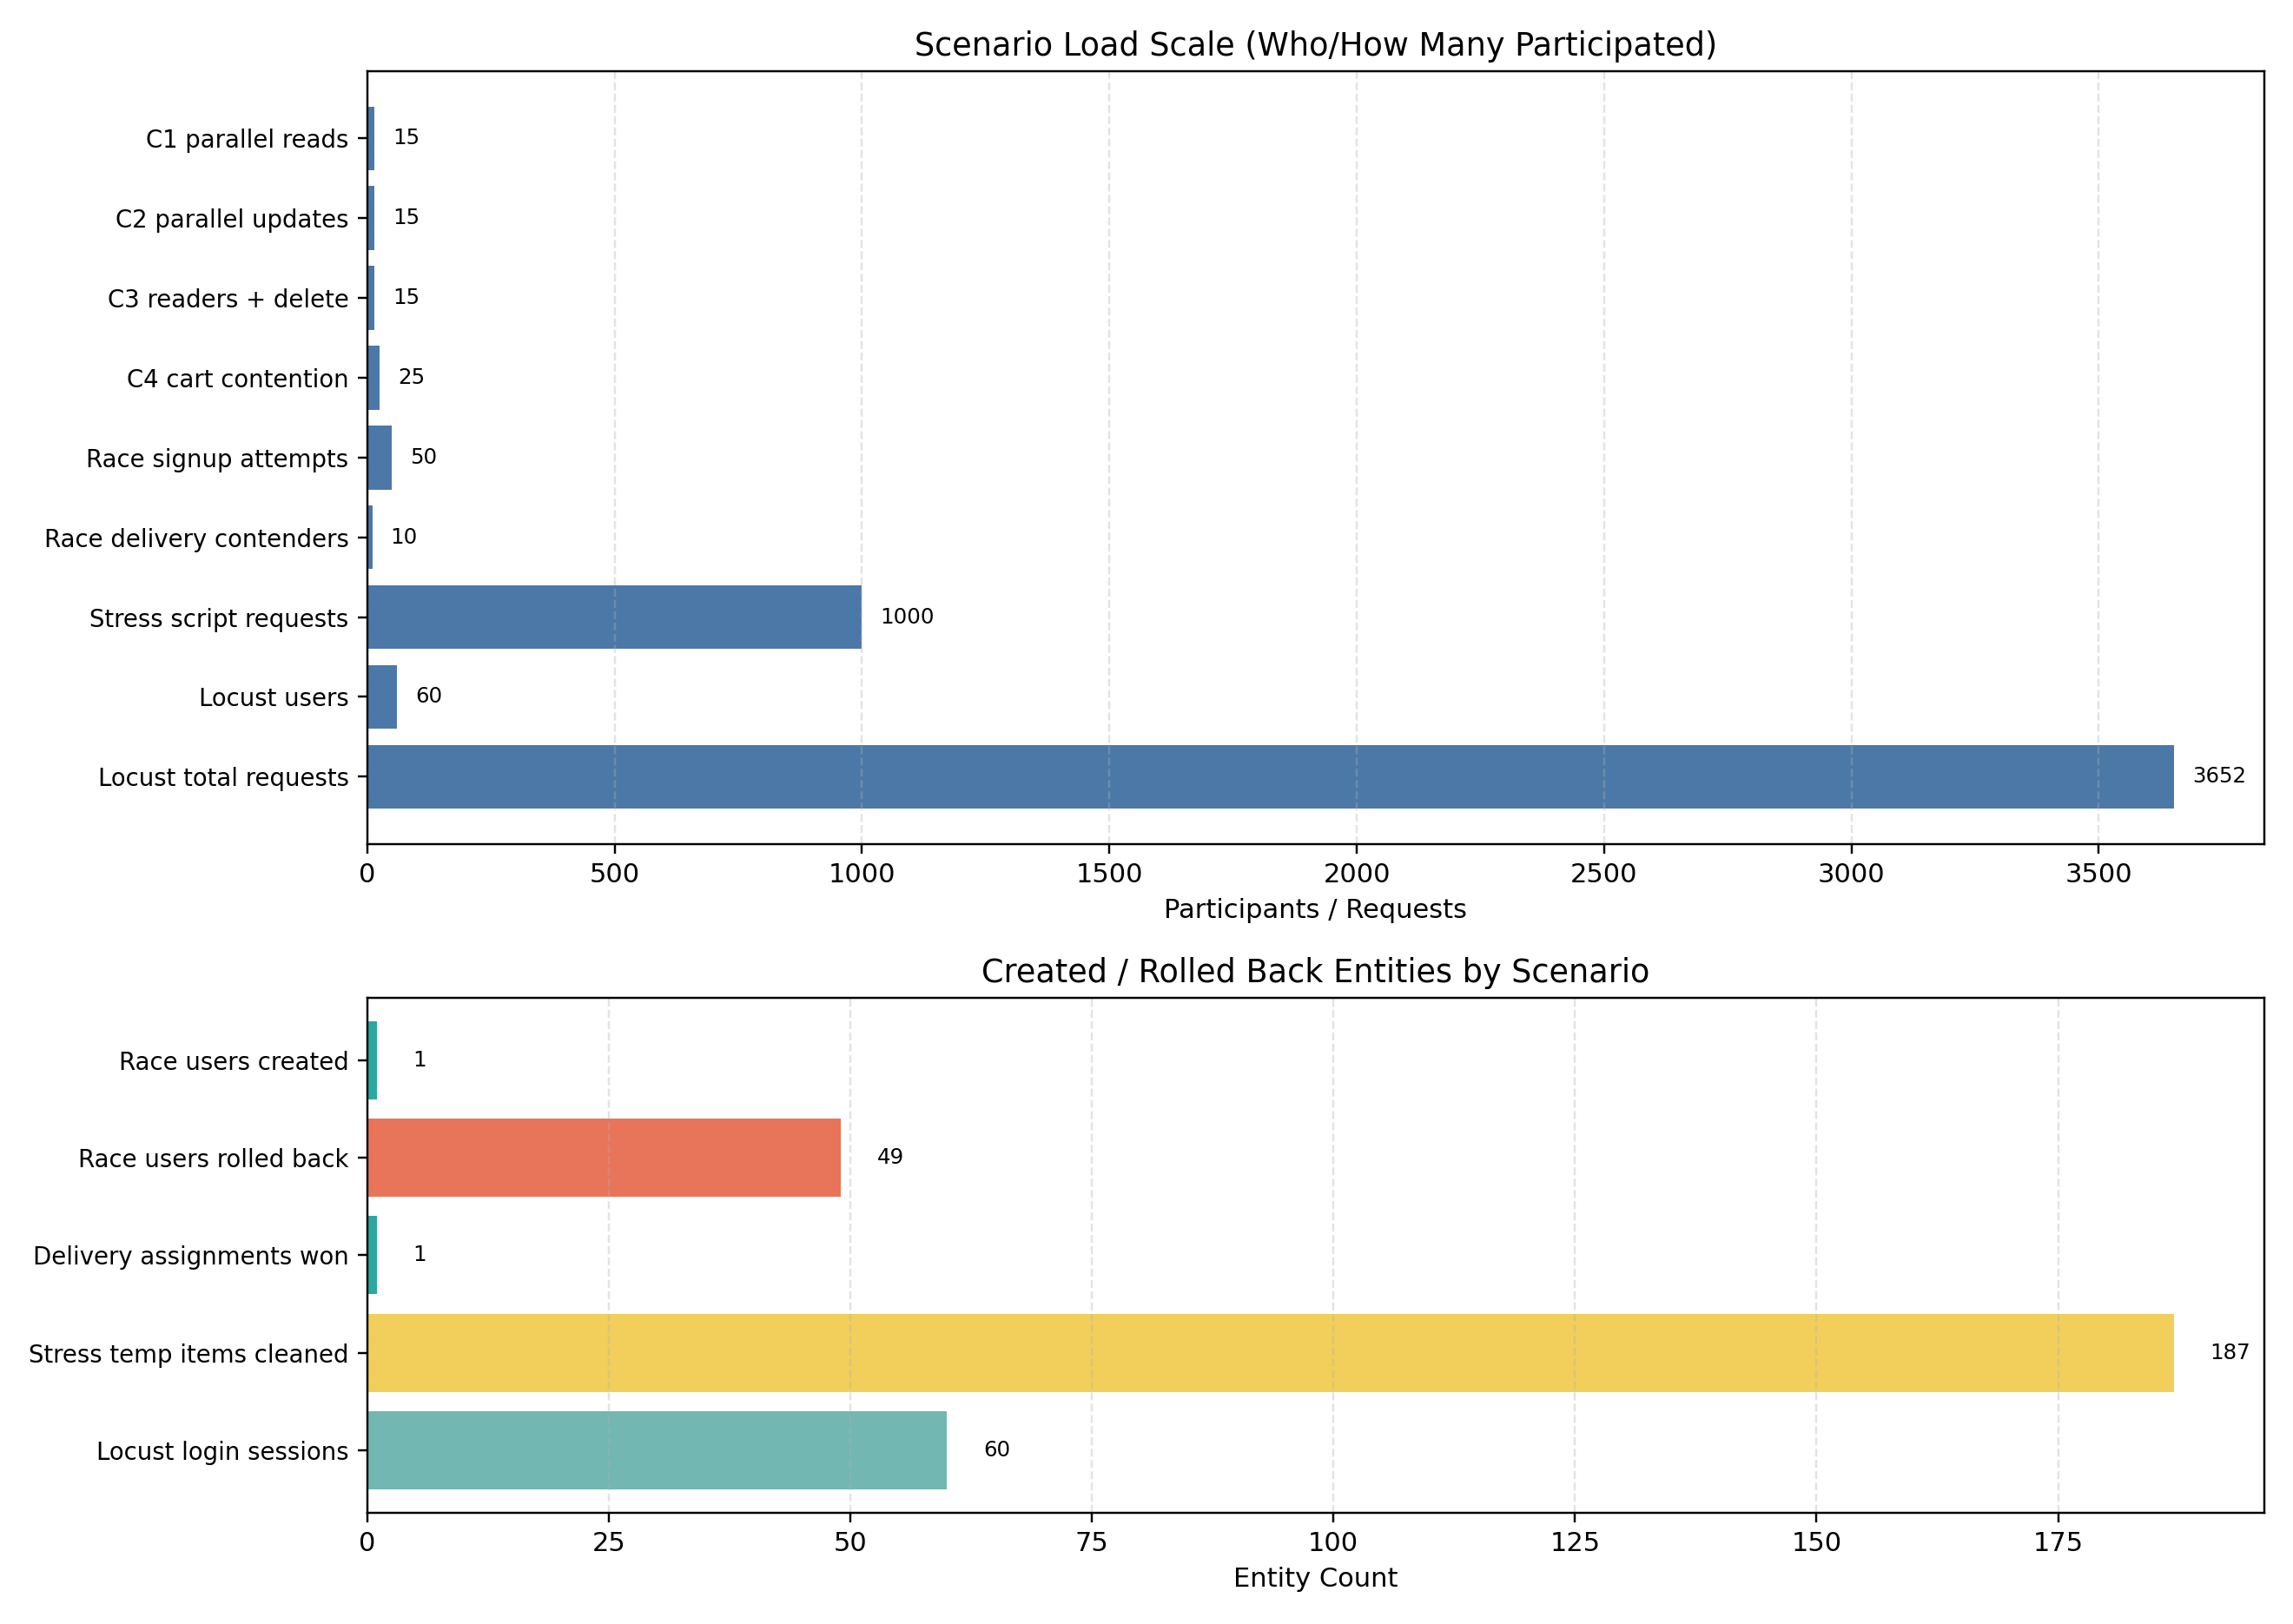
\includegraphics[width=0.84\textwidth]{../figures/test_cases/test_duration_by_case_ms.png}
    \caption{Figure 2: Scenario load scale and entity outcomes (participants, attempts, and created or rolled-back records).}
\end{figure}

\begin{figure}[h]
    \centering
    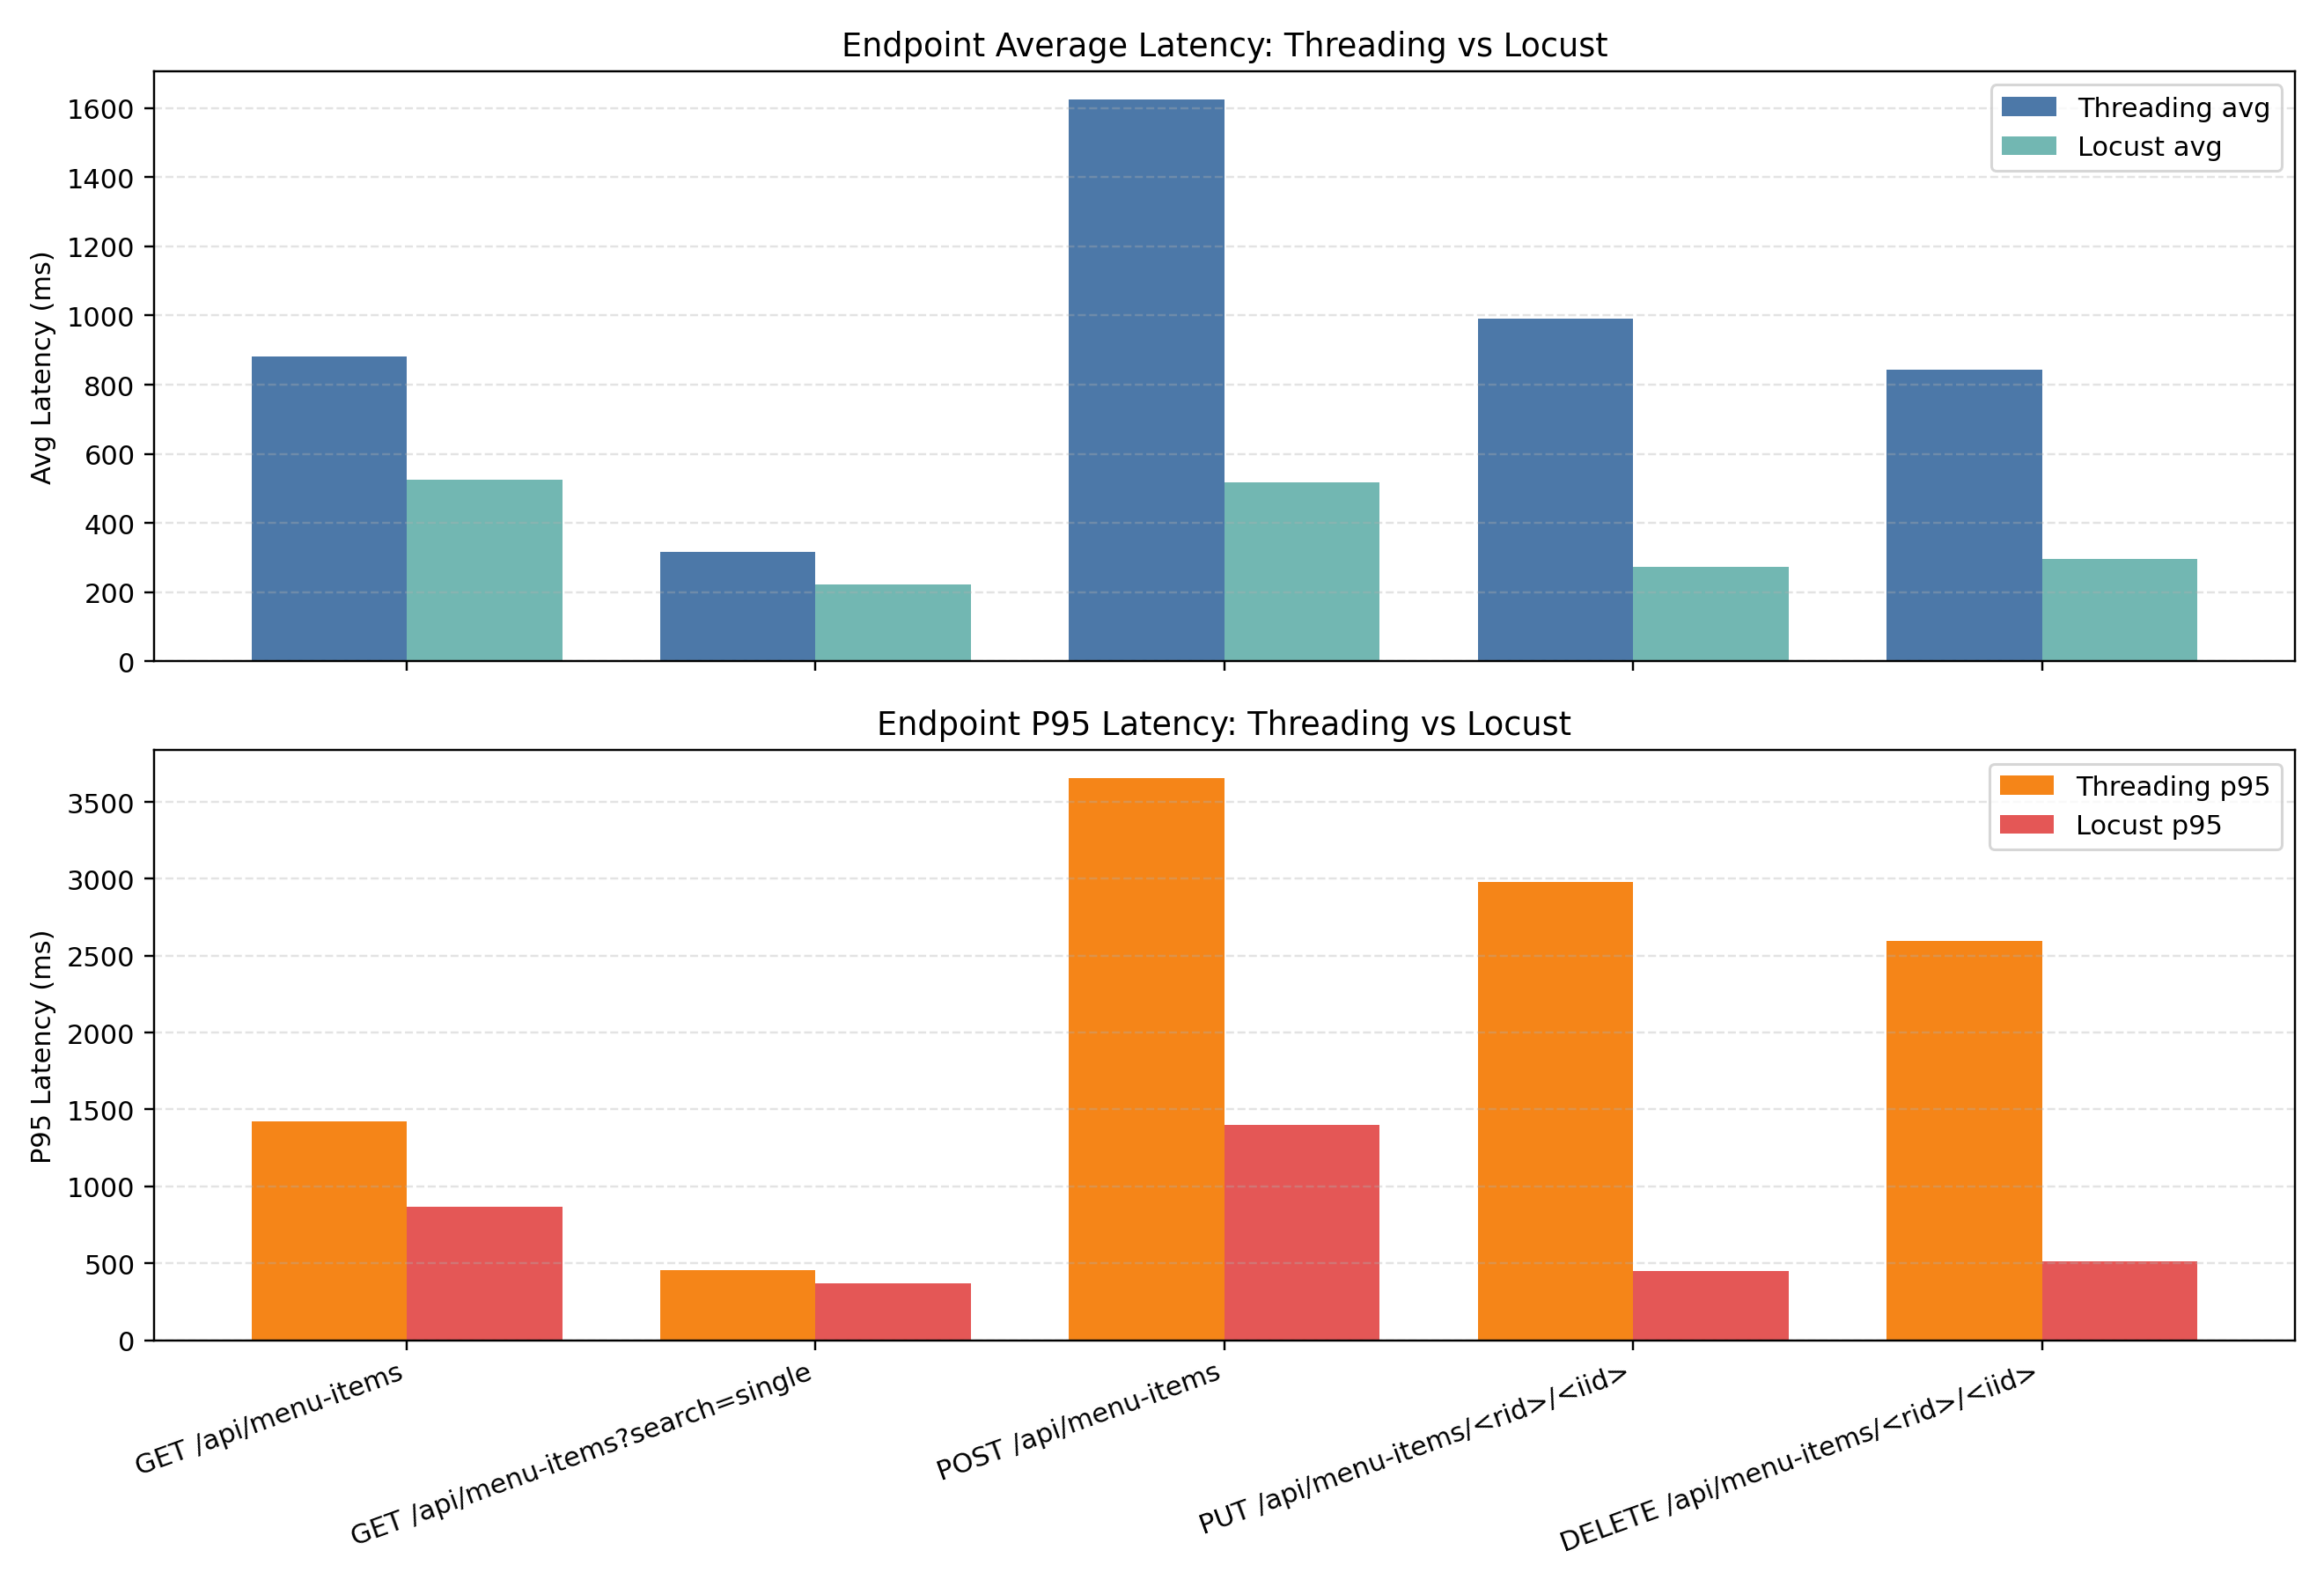
\includegraphics[width=0.84\textwidth]{../figures/test_cases/stress_endpoint_metrics.png}
    \caption{Figure 3: Endpoint latency comparison under stress (threading vs Locust, average and p95).}
\end{figure}

\clearpage
\section{Discussion}
The latest execution indicates strong transactional correctness across concurrent, race, failure, and ACID suites. All suites reported complete pass status with no residual integrity anomalies. Under stress, correctness remained stable (0\% errors in both threading and Locust runs), but write-heavy operations exhibit materially higher tail latency than read-oriented operations. This pattern is consistent with lock contention and transaction serialization on critical write paths.

Locust appears faster than the threading stress script primarily because workload shape differs: Locust applies user think-time and distributed task pacing, while the threading script continuously drives requests with fixed worker concurrency and more sustained contention bursts. Therefore, Locust and threading values should be interpreted as complementary profiles, not direct one-to-one latency replacements.

\section{Reproducibility}
Latest verification can be reproduced with:
\begin{verbatim}
python tests/concurrent_test.py
python tests/race_condition_test.py
python tests/failure_simulation_test.py
python tests/acid_verification.py
python tests/stress_test.py
locust -f locustfile.py --headless -u 60 -r 20 -t 1m --host http://127.0.0.1:5001
\end{verbatim}

To build this report via LaTeX:
\begin{verbatim}
make report-latex
\end{verbatim}

\section{Conclusion}
The backend demonstrates required transactional reliability properties for this assignment: operations complete atomically, inconsistent partial states are prevented, concurrent users are isolated in critical workflows, and committed data survives restart conditions. System robustness under load is acceptable for assignment scope, with clear optimization targets identified around high-percentile write latency and lock-heavy update paths.

\end{document}